
% Introduction to the different properties of a reservoir to be benchmarked.
Before attempting to solve a specific computational task, it is important to 
map out what the physical reservoir can do by benchmarking its computational properties.
To have computational capacity, a reservoir should show input separability and fading memory \citep{nakajima_information_2015}.
Evaluating these properties is in fact a way of characterizing the echo response function of the system as described in Section \ref{section:rc-general}.
% To determine the computational capacity of a reservoir, we must evaluate it on three key fronts: (i) input separability; (ii) fading memory property; (iii) memory capacity \citep{nakajima_information_2015, nakajima_physical_2020}.

% Q: add (iv) stationarity?

\subsection{Input Separability}

% What is input separability
The readout function is a strictly linear model. 
To solve nonlinear tasks, the reservoir must transform its inputs such that the task becomes a linear function of the reservoir state.
In other words, there must be a linear relation between the reservoir's observable state and the target task.
Figure \ref{fig:input_sep_principle} shows an example of linear input separation in a reservoir.

However, the nonlinear transformation applied by a finite reservoir cannot solve any arbitrary task.
In addition, the presence of notable recurrent effects in the reservoir may degrade precision in recalling recent inputs (Section \ref{section:rc-time-scales} explores this phenomenon further).
When the input transformation applied by the reservoir results in an observable state from which a readout function can compute the desired task efficiently, we speak of good input separability.
Good input separability is a function of both nonlinearity and memory, and the optimal mix of both properties varies depending on the task.


% How to measure input separability
One way to evaluate the input separation of a reservoir relative to a given task is to train a reservoir readout and a control readout model \citep{ushio_computational_2021}. 
The former fits to the reservoir state, while the latter fits to the environmental signals directly.
If the expanded state of the reservoir contains helpful input separation for the task, the reservoir readout will perform better than the control model.


\subsection{Fading Memory} \label{sec:fading_memory}

% Introduction to fading memory
Section \ref{section:esp} already stated the importance of fading memory in physical reservoirs.
However, this property is difficult to measure directly.
Nonetheless, we will outline two ideas for measuring this property in physical systems.


% Method 1: warmup time
The first method attempts to measure the warmup time of the reservoir. 
The idea is simple: initialize the same reservoir with different starting conditions, then measure the time it takes for the reservoir state to synchronize to the input.
If the physical system displays the fading memory property, then the trajectories of the reservoirs will eventually synchronize, even if initialized with different starting conditions.
Figure \ref{fig:memory_esn_start} demonstrates this method on an \acrshort{esn} with different leak rates. 
In this experiment, An \acrshort{esn} is subjected to identical input series with two different initial reservoir states $\mathbf{x}$.
The rate at which the reservoir syncs to the input signal depends on the time scale of the reservoir dynamics dictated by the leak rate.

% Method 2: signal spike
In the second method, we subject two reservoirs to identical input signals. 
One reservoir will serve as the test subject, while the other acts as a control.
After the two systems have synchronized to the input, we briefly apply an environmental impulse to the test reservoir, after which the original input signal resumes.
We then measure the time for the test reservoir to resynchronize with the control reservoir.
This impulse can look different depending on the type of reservoir. 
For example, we can temporarily remove the reservoir from its environment such that it no longer receives any environmental stimuli.
Another possibility is to apply an unexpected and artificial stimulus for a short time.
Regardless of how we realize the impulse, we must apply it long enough to have a noticeable impact on the trajectory of the reservoir dynamics.
Otherwise, it is impossible to measure the time until the reservoir synchronizes to the regular inputs.
Figure \ref{fig:memory_esn_impulse} demonstrates this method on an \acrshort{esn}.
This time, all input values between time steps 60 and 80 are set to a fixed value of ten times the standard deviation of the input signal.
After step 80, the reservoir gradually returns to its original behavior, at a rate proportional to its leak rate.


% Measuring divergence in trajectories
Both methods rely on measuring the divergence in behavior of a reservoir when subjected to different conditions. 
To quantitatively compare the difference between reservoir states at time $t$, we can use a distance metric such as \acrfull{mse} on its observable state $X$:

\begin{equation} \label{eq:MSE}
    \text{MSE}(t) = \frac{1}{N} \sum_{i=1}^{N} \left( X_i^{(1)}(t) - X_i^{(2)}(t) \right)^{2}
\end{equation}

where $N$ is the size of the reservoir's observable state vector.


% Relation to memory capacity.
Note that in both experiments, the time it takes for the reservoirs to synchronize also informs about its recurrent dynamics and memory capacity.

\begin{figure}
    \centering
    \begin{subfigure}[b]{0.485\linewidth}
        \centering
        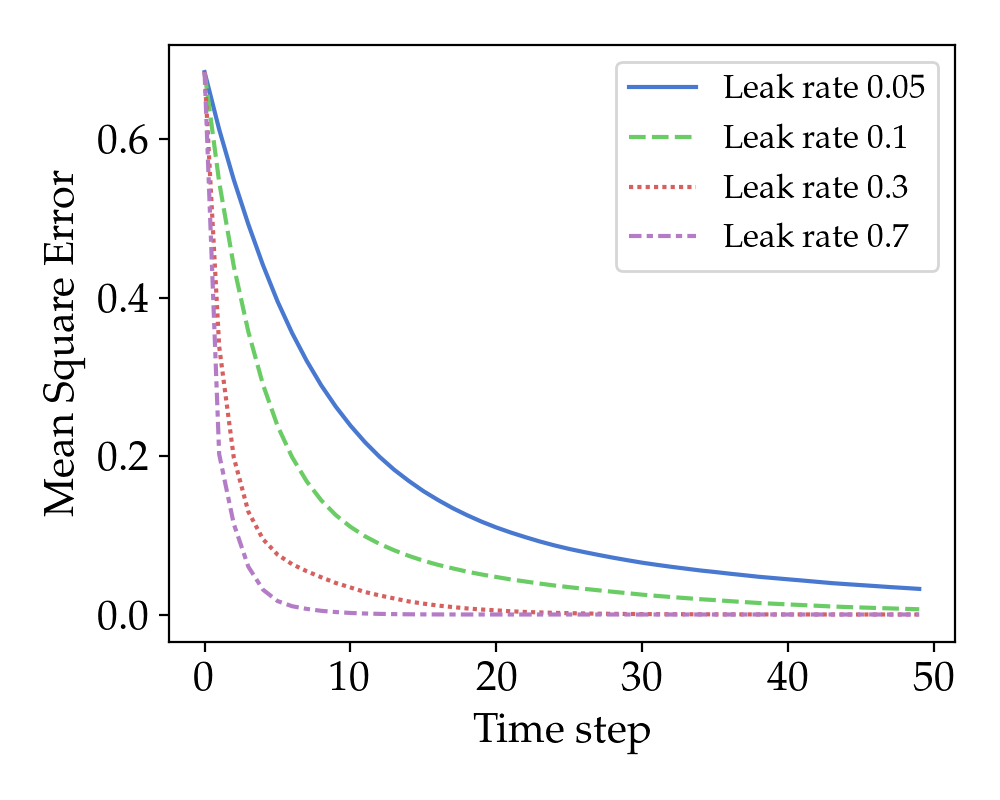
\includegraphics[width=\linewidth,height=\linewidth,keepaspectratio]{img/esn_starting_conditions.png}
        \caption{First method: divergence between reservoirs}
        \label{fig:memory_esn_start}
    \end{subfigure}
    \vskip\baselineskip
    \begin{subfigure}[b]{0.485\linewidth}
        \centering
        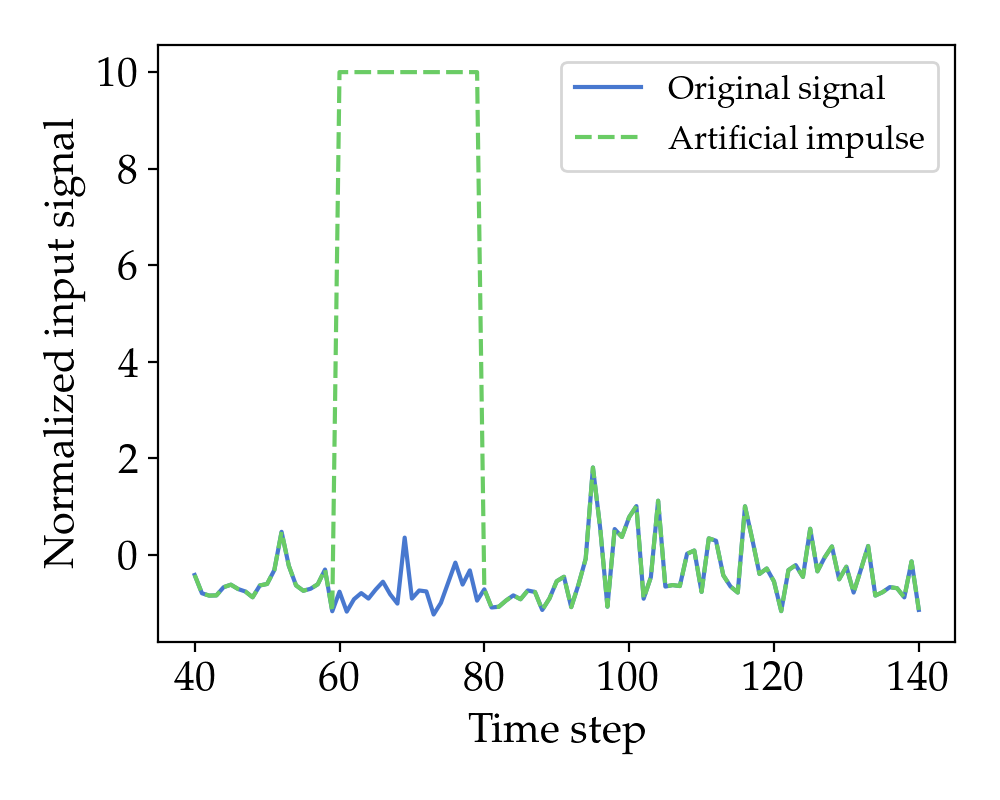
\includegraphics[width=\linewidth,height=\linewidth,keepaspectratio]{img/input_impulse.png}
        \caption{Second method: applying an artificial impulse}
        \label{fig:memory_input_impulse}
    \end{subfigure}
    \hfill
    \begin{subfigure}[b]{0.485\linewidth}
        \centering
        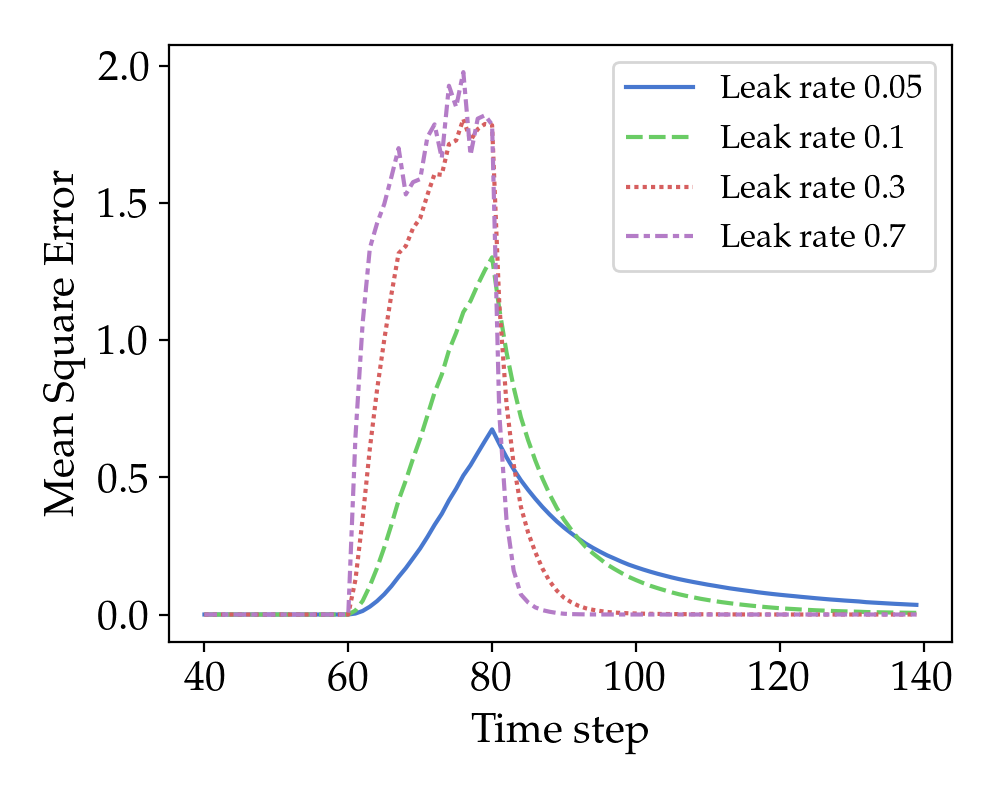
\includegraphics[width=\linewidth,height=\linewidth,keepaspectratio]{img/esn_impulse.png}
        \caption{Second method: divergence between reservoirs}
        \label{fig:memory_esn_impulse}
    \end{subfigure}
    \caption[Two methods for testing the fading memory property of a reservoir, demonstrated using a \acrshort{esn}.]{
            These figures show experimental data from testing the fading memory property of an \acrshort{esn} as described in Subsection \ref{sec:fading_memory}. 
            Both experiments use a reservoir of 100 nodes with randomly initialized weights. 
            For stability, we normalized the weights to have a spectral radius below 1.25 \citep{caluwaerts_design_2014}.
            As input data, we used the California Housing regression dataset \citep{kelley_pace_sparse_1997} which can be found in the sklearn Python package.
            (\subref{fig:memory_esn_start}) The divergence in reservoir state between two runs of the same reservoir with identical inputs and different starting state vectors. 
            The starting states are sampled from a uniform distribution between -1 and 1.
            The disparity between the reservoirs is measured by the MSE between their respective state vectors (Equation \ref{eq:MSE}).
            (\subref{fig:memory_input_impulse}) An artificial impulse with an amplitude of ten times the standard deviation of the original signal is applied between time steps 60 and 80.
            (\subref{fig:memory_esn_impulse}) The divergence in reservoir state between two runs of the same reservoir using identical starting conditions. One run receives an artificial impulse between time step 60 and 80 on all input dimensions, as depicted by Subfigure \subref{fig:memory_input_impulse}.
    }
    \label{fig:fading_memory_experiments}
\end{figure}



\subsection{Computational Benchmarks}

% NARMA
To better compare results between studies of different reservoirs, some standard benchmarks appear in the literature.
The most common \acrshort{rc} benchmark is the nonlinear autoregressive moving average (\acrshort{narma}).
We can tune the nonlinearity and memory of the \acrshort{narma} task With the $n$ parameter.
The \acrshort{narma} system is defined as:

\begin{equation} \label{prc:narma}
    y(t+1) = \alpha y(t) + \beta y(t) \left[ \sum_{i=0}^{n-1} y(t-i) \right] + \gamma x(t-n+1) x(t) + \delta
\end{equation}

where the parameters $\alpha$, $\beta$, $\gamma$, and $\delta$ are set to 0.3, 0.05, 1.5 and 0.1 \citep{nakajima_information_2015}.

For some reservoirs, it is necessary to tune the NARMA system's memory to the correct time scale to get stable results \citep{pieters_reservoir_2022}.
For this the adapted formula can be used:

\begin{equation} \label{prc:narma-timescale-adapted}
    y(t+1) = \alpha y(t) + \beta y(t) \left[ \sum_{i=0}^{n-1} y(t-\tau i) \right] + \gamma x(t-\tau n+1) x(t) + \delta
\end{equation}

where $\tau$ is tuned to the desired time scale of the NARMA system's memory.


% Delay line and polynomial expansion
We can use other simple benchmarks to evaluate the memory and nonlinear properties.
For example, predicting the past inputs of the reservoir for increasing delay tests the memory of the system:

\begin{equation} \label{prc:delay-line-benchmark}
    y(t) = x(t-\tau)
\end{equation}

where greater values of $\tau$ require more memory to solve ($\tau > 0$). 
To test reservoir nonlinearity, a simple exponentiation of the input signal can be used as the prediction target:

\begin{equation} \label{prc:polynomial-benchmark}
    y(t) = (x(t))^{n}
\end{equation}

where $n$ is greater or less than 1.


% Chaotic systems
Finally, to test a reservoir's ability to predict the trajectory of chaotic systems, \citet{ushio_computational_2021} have proposed a test using strange attractors.
In this test, a time series of a Lorenz attractor acts as the input to the reservoir.
The reservoir then has to predict near-future values of this input time series.
The test evaluates how well the reservoir can synchronize with a chaotic system, which is a common application for \acrshort{rc} \citep{tanaka_recent_2019}.
